\chapter{RRDtool as a Communication}

\section{Introduzione}

Quello che abbiamo visto fino ad adesso è relativo ai cosiddetti ``\textit{elements}'', ovvero ai componenti di rete che in sostanza permettono che funzioni.\

Quello che possiamo fare è di studiare se il traffico è più o meno aspettato nei volumi:\ non possiamo investigare nei contenuti quindi non possiamo sapere il tipo del traffico, ma possiamo conoscerne i volumi.\
Possiamo studiare lo stato delle porte per sapere se c'è una disconnessione, se c'è una riconnessione e sapere se c'è qualcuno che si è spostato o ha abbandonato la rete.\
Questo, sopratutto per la sicurezza, è un aspetto importante.\
C'è la necessità di sapere se avviene un cambiamento, di capire il tipo di periferica e di come quest'ultima sia collegata alla rete.\

Tramite il Bridge MIB è possibile andare a scoprire dove le device siano effettivamente connesse:\ per monitorare una rete è importante non solo vedere il traffico ma assicurarci che venga da dove ci aspettiamo.\
Infine, tramite LLDP è possibile conoscere la topologia di una rete.\

\begin{center}
    I dati raccolti tramite SNMP dove vengono memorizzati?
\end{center}

\section{RRD}

I database relazionali sono nati per supportare operazioni di inserimento, cancellazione e modifica dei dati.\
Nel mondo delle reti, e anche in altri mondi, queste operazioni non sono ``normali'':\ le cancellazioni, come le modifiche, sono proibite;
inoltre, quando la cardinalità del numero di righe per tabella aumenta sopra un certo livello, la dimensione dei file contenenti gli indici delle entries, i quali sono utilizzati proprio per velocizzare le operazioni di modifica, può diventare più grande di quella del contenuto stesso.\
Se si monitorasse lo stato di una porta a intervalli di un minuto, che ci sia traffico o meno, si scriverebbero $60 \times 24$ righe all'interno di una tabella in un solo giorno.\
Se poi si considera il monitoraggio di un intero switch, è impensabile utilizzare un database SQL per memorizzare tutti i dati raccolti.\

È necessario poter consolidare, raggruppare, i dati più vecchi per ottenere molteplici tipi di vista con granularità differente cosicché la dimensione su disco sia minore.\

\vspace{12pt}
\noindent L'RRD (\textit{Round Robin Database}) ha una dimensione di archiviazione prefissata:\ periodicamente si va a scrivere in uno slot e quando si terminano gli slot a disposizione, si va sovrascrivere il primo, ottenendo la cosiddetta ``\textit{sliding window}''.\

\begin{figure}[H]
    \centering
    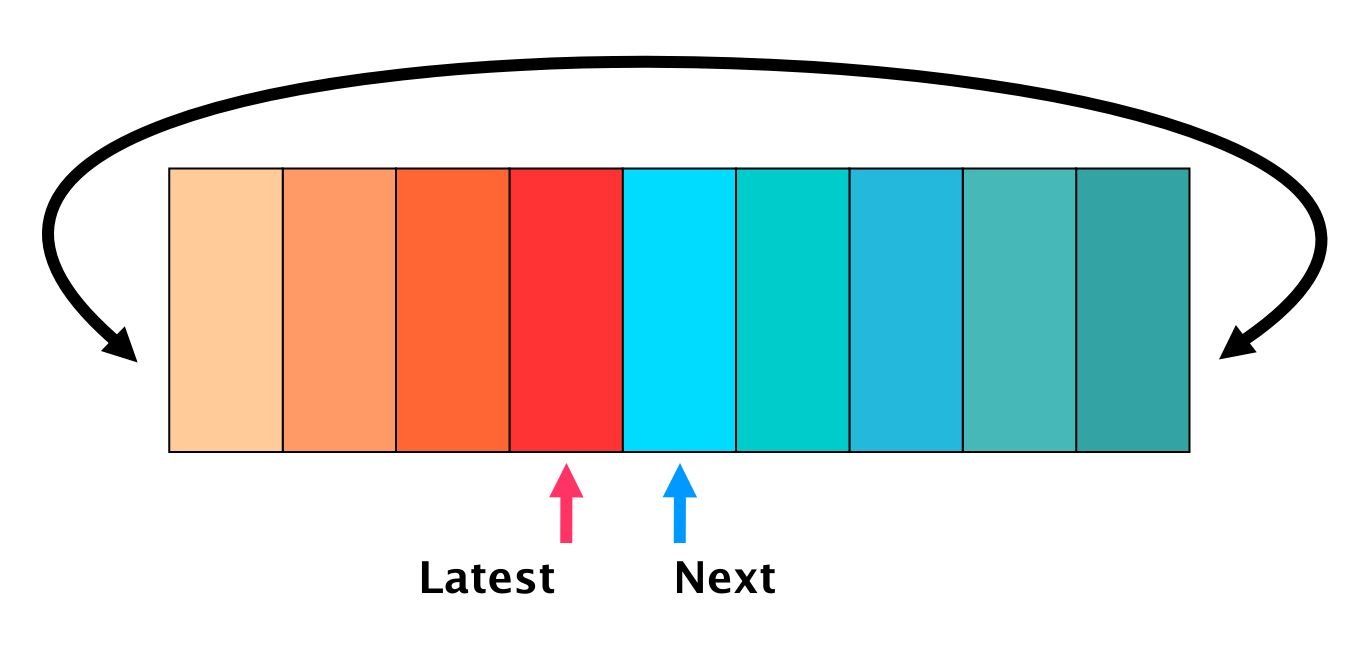
\includegraphics[width=0.8\textwidth]{immagini/RRD.png}
\end{figure}

\noindent Componenti di un file RRD

\begin{itemize}
    \item Header statico:\ contiene il nome del file, un contatore di byte, un contatore di pacchetti,\ \dots
    \item Live Header:\ è dove vengono contenuti gli indici; mantiene l'indice e il contenuto dell'ultimo slot scritto.
    \item Archivi RRA:\ spazi che contengono una metrica; quando scrivo sul database, scrivo su tutti gli archivi.
\end{itemize}

\noindent Che cos'è un Data Source?\ Quali sono le sorgenti dei dati a cui si attinge per scrivere in RRD?\
``Una qualsiasi cosa che sia numerica'':\ file di log, contatori SNMP, \verb|/proc| entries, output da un programma,\ \dots

\subsubsection{Gestione di un dato sconosciuto}

Se per qualche motivo non avviene una scrittura su un database che dovrebbe essere aggiornato periodicamente, non è possibile usare il valore `0', ma è necessario indicare il valore come \textbf{sconosciuto}.\

\begin{center}
    ``\textit{Sconosciuto}'' è contagioso:\  1 + Sconosciuto = Sconosciuto
\end{center}

\noindent RRD permette di gestire situazioni in cui si è ``persa'' una scrittura a causa dello scostamento accumulato nel tempo.\

\subsubsection{Archivi multipli}

I file RRD possono contenere più archivi:\ è possibile inserire più metriche diverse (byte, pacchetti), oppure la stessa metrica a risoluzione diversa.\
Al momento della creazione del database va indicato quanto è granulare il dato che sarà inserito e come fare le eventuali aggregazioni.

